\chapter{Architecture}

\section{External Architecture}

The Biobank application uses a hexagonal architecture to interface to internal
and external clients, external services, and for data storage. Figure
\ref{fig:hex-architecture} shows the how the ports are configured. Web browser
based clients access the application via the internal client port. A RESTful
interface is also supported to allow the Biobank scanning client access via the
external client port. External systems can also access the application via this
port. Biobank can communicate to external services by using the external
services port. The figure also shows that the event store and query databases
are accessed via dedicated ports.

\begin{figure}[h]
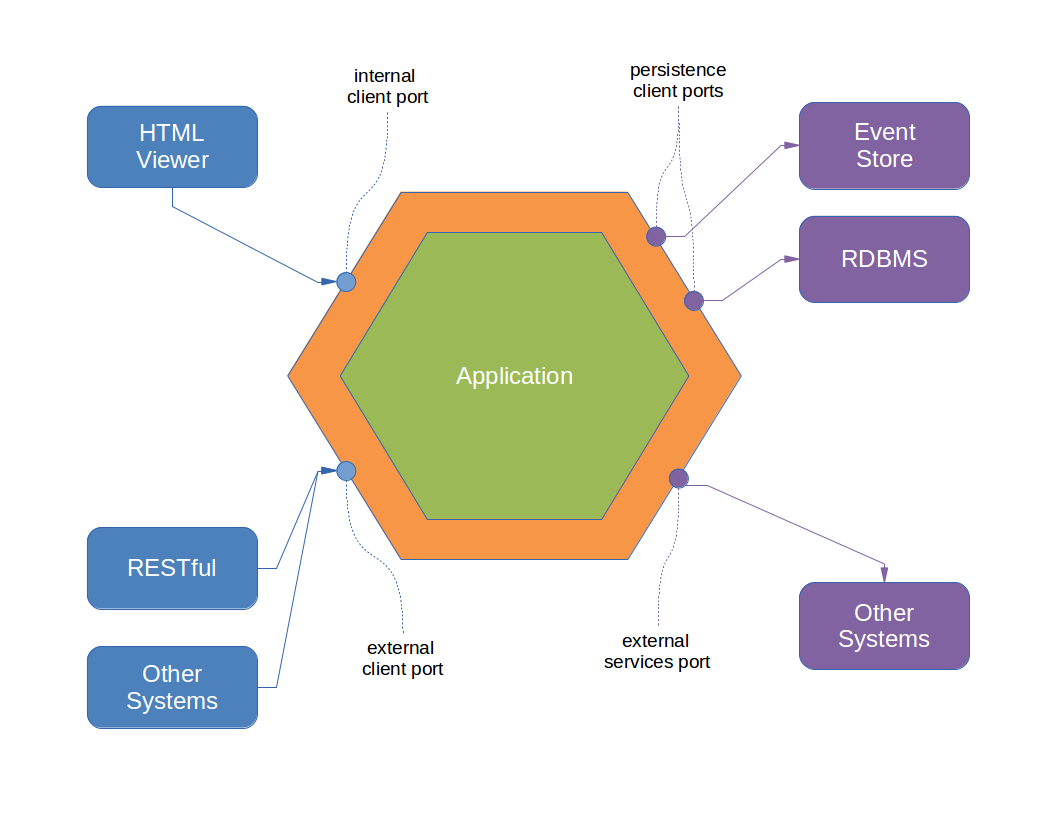
\includegraphics[width=1\textwidth]{images/hex-architecture}
\caption{Hexagonal architecture}
\label{fig:hex-architecture}
\end{figure}

\section{Interal Architecture}

The client ports shown in Figure \ref{fig:hex-architecture} are managed by
client adapters. These client adapters then interface to the rest of the system
via \emph{Command Handlers} and the \emph{Query Interface}. Figure
\ref{fig:cqrs-architecture} shows a more detailed view of the application. It
is the architecture recommended by the Axon Framework\footnote{The figure and
  the material that follows is borrowed from the Axon Framework Reference Guide
  \cite{AxonOnline}}.

\begin{figure}[h]
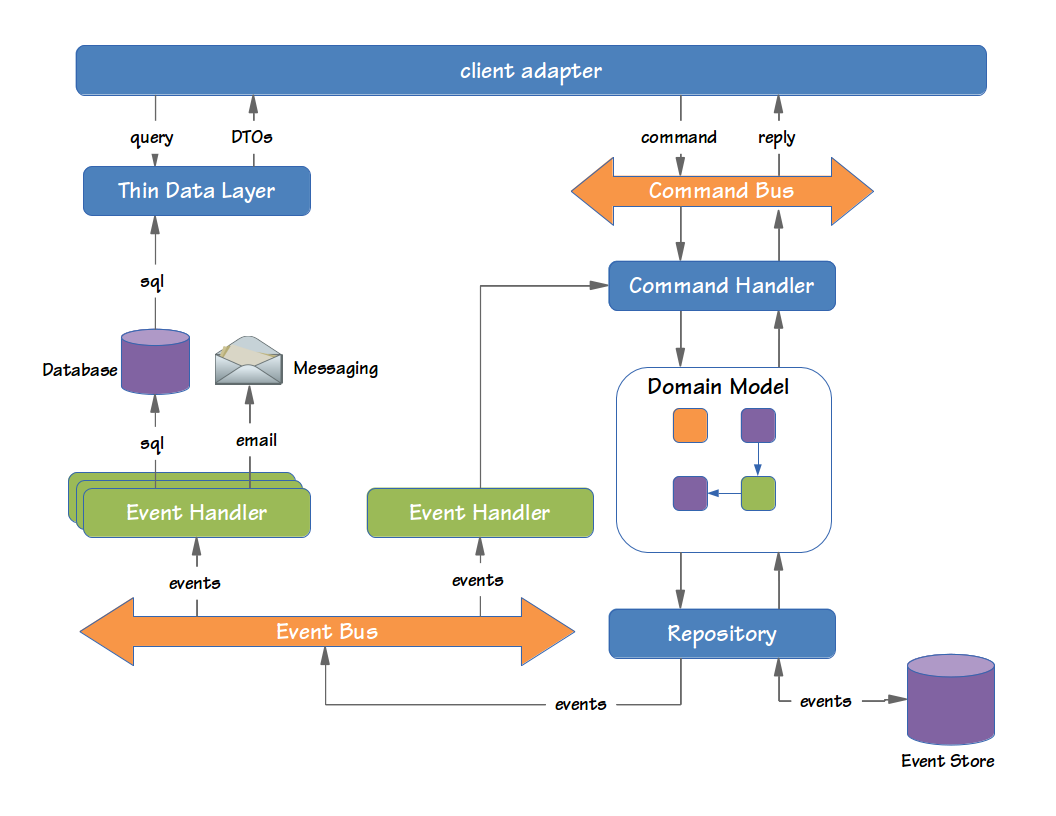
\includegraphics[width=0.95\textwidth]{images/cqrs-architecture}
\caption{Biobank application architecture}
\label{fig:cqrs-architecture}
\end{figure}

\section*{Command Handling}

Commands are typically represented by simple and straightforward objects that
contain all data necessary for a command handler to execute it. A command
expresses its intent by its name. In Java terms, that means the class name is
used to figure out what needs to be done, and the fields of the command provide
the information required to do it.

The Command Bus receives commands and routes them to the Command Handlers. Each
command handler responds to a specific type of command and executes logic based
on the contents of the command. In some cases, however, logic is executed
regardless of the actual type of command, such as validation, logging or
authorization.

\section*{Domain Model}

The command handler retrieves domain objects (Aggregates) from a repository and
executes methods on them to change their state. These aggregates typically
contain the actual business logic and are responsible for guarding their own
invariants. The state changes of aggregates result in the generation of Domain
Events. Both the Domain Events and the Aggregates form the domain model.

\section*{Repositories and Event Stores}

Repositories are responsible for providing access to aggregates. Typically,
these repositories are optimized for lookup of an aggregate by its unique
identity. Repositories store the state changes that the aggregate has gone
through in an Event Store. The repository is also responsible for persisting
the changes made to aggregates in its backing storage.

\section*{Event Processing}

The event bus dispatches events to all interested event handlers. This is done
synchronously or asynchronously. Asynchronous event dispatching allows the
command execution to return and hand over control to the user, while the events
are being dispatched and processed in the background. Not having to wait for
event processing to complete makes an application more responsive. Synchronous
event processing, on the other hand, is simpler and is a sensible
default. Synchronous processing also allows several event listeners to process
events within the same transaction.

Event handlers receive events from the event bus. Some handlers update data
sources used for querying while others send messages to external
systems. Command handlers are completely unaware of the components that are
interested in the changes they make. This means that it is very non-intrusive
to extend the application with new functionality. All you need to do is add
another event handler. The events loosely couple all components in your
application together.

In some cases, event processing requires new commands to be sent to the
application. The saga is the CQRS concept responsible for managing these
complex business transactions.

\section*{Querying for data}

The thin data layer in between the client adapters and the data sources
provides a clearly defined interface to the actual query implementation
used. This data layer typically returns read-only Data Transfer Objects (DTOs)
containing query results. The contents of these DTOs are typically driven by
the needs of the client adapters. In most cases, they map directly to a
specific view in the UI (also referred to as table-per-view).

\subsection{Axon Framework Modules}

The Axon Framework provides a number of different modules that target specific
problem areas of CQRS. This section describes which modules were chosen.

\todo[size=\small]{complete this section}
